%%%%%%%%%%%%%%%%%%%%%%%%%%%%%%%%%%%%%%%%%%%%%%%%%%%%%%%%%%%%%%%%%%%%%%%%%%%%
% What the code does and how to use it:
% Code takes the countyr data from the files generated by 
% read_UNPD_fertility_data.py and read_UNPD_mortality_data.py
% (e.g. ZimbabweMortalityMen_WPP2017.csv and ZimbabweMortalityWomen_WPP2017.csv)
% and fits regression models (over time) for each gender+age group.
% Code outputs files called e.g. Zimbabwe_mortalityByAgeCoefficients.txt 
% These files can go straight into the PopART IBM (rename to param_mortality.txt).
% Note - the code also runs regression for fertility - this shows that we SHOULDN'T USE REGRESSION FOR FERTILITY (WE USE THE ORIGINAL UNPD NUMBERS). It also runs an 'experiment' where we try to create a smaller regression model (rather than stratifying by age, we use the model mortality ~ (age + time)) - this does not seem to produce good fits so I ignore it.

% HOW TO RUN THE CODE:
% 1) modify the country variable to the right country
% 2) modify the UNPD WPP edition ('unpd.version')
% 3) Check that you have the UNPD files genrated by read_UNPD_mortality_data.py and read_UNPD_fertility_data.py
% 4) Run the code:
% R CMD Sweave EstimatingRatesFromUNPDv2.Rnw 
% pdflatex EstimatingRatesFromUNPDv2.tex 
% 5) View the file EstimatingRatesFromUNPDv2.pdf. IMPORTANT: check that the graphs on pages 2-5 (mortality curve fitted to UNPD) adequately fits the UNPD mortality data, excluding any bump due to HIV. At present I fit to the first 7 timepoints (i.e. 1952.5-1982.5) and the last 13 points (2032.5-2097.5 I think) but can also fit to more or less data. To change this, modify the parameter 'mortality.years.to.use'.
% If you're happy then use the file called COUNTRY_mortalityByAgeCoefficients.txt as your param_mortality.txt.

%%%%%%%%%%%%%%%%%%%%%%%%%%%%%%%%%%%%%%%%%%%%%%%%%%%%%%%%%%%%%%%%%%%%%%%%%%%%
%%%% Validation of code:
% Ran using existing (i.e. the original ones I copied by hand, not the ones generated by read_UNPD_mortality_data.py) SouthAfrica_mortalityByAgeCoefficients.txtand Zambia_mortalityByAgeCoefficients.txt. Compared them to the ones sources by the IBM:  ~/popart-ibm-code/popart-code/IBM_simul/RAW_PRIORS/SOURCED_FROM_LITERATURE/Analysing_UNPD_estimates_demographic_params/SouthAfrica_mortalityByAgeCoefficients.txt  and Zambia_mortalityByAgeCoefficients.txt .
% Outputs are a perfect match.
%%%%%%%%%%%%%%%%%%%%%%%%%%%%%%%%%%%%%%%%%%%%%%%%%%%%%%%%%%%%%%%%%%%%%%%%%%%%


\documentclass{article}

%%% Choosing the margins of the document %%%
\usepackage{geometry}
\geometry{a4paper, portrait, margin=1in}
%%% Package to make sure figures are in right section %%%
\usepackage[section]{placeins}
%%% package for colours
\usepackage{color}
\usepackage{lscape}

\usepackage{Sweave}
\begin{document}
\Sconcordance{concordance:EstimatingRatesFromUNPDv2.tex:/home/mike/MANICALAND/manicaland-dev/Parameterization/Demographics/EstimatingRatesFromUNPDv2.Rnw:%
1 37 1 1 0 9 1 1 38 3 1 1 37 2 1 1 25 1 1 1 26 3 0 1 6 1 2 2 1 1 20 2 1 %
1 24 3 0 1 6 1 2 40 1 1 3 12 0 1 1 12 0 1 3 7 1 1 3 6 0 1 3 5 1 1 20 15 %
1 1 22 14 1}


%%% Some options to make the R code look nicer in Sweave %%%
\DefineVerbatimEnvironment{Sinput}{Verbatim} {xleftmargin=2em}
\DefineVerbatimEnvironment{Soutput}{Verbatim}{xleftmargin=2em}
\DefineVerbatimEnvironment{Scode}{Verbatim}{xleftmargin=2em}
\fvset{listparameters={\setlength{\topsep}{0pt}}}
\renewenvironment{Schunk}{\vspace{\topsep}}{\vspace{\topsep}}

%%%%%%%%%%%%%%%%%%%%%%%%%%%%%%%%%%%%%%%%%%%%%%%%

\section*{Mortality rates}



% Plot male mortality in younger age groups (age 0-44)

% Plot male mortality in older age groups (age 45+)
\begin{Schunk}
\begin{Soutput}
NULL
\end{Soutput}
\end{Schunk}


% Plot female mortality in younger age groups (age 0-44)


% Plot female mortality in older age groups (age 45+)
\begin{Schunk}
\begin{Soutput}
NULL
\end{Soutput}
\end{Schunk}


%%%%%%%%%%%%%%%%%%%%%%%%%%%%%%%%%%%%%%%
%%%%%%%%%%%%%%%%%%%%%%%%%%%%%%%%%%%%%%%%

\begin{figure}
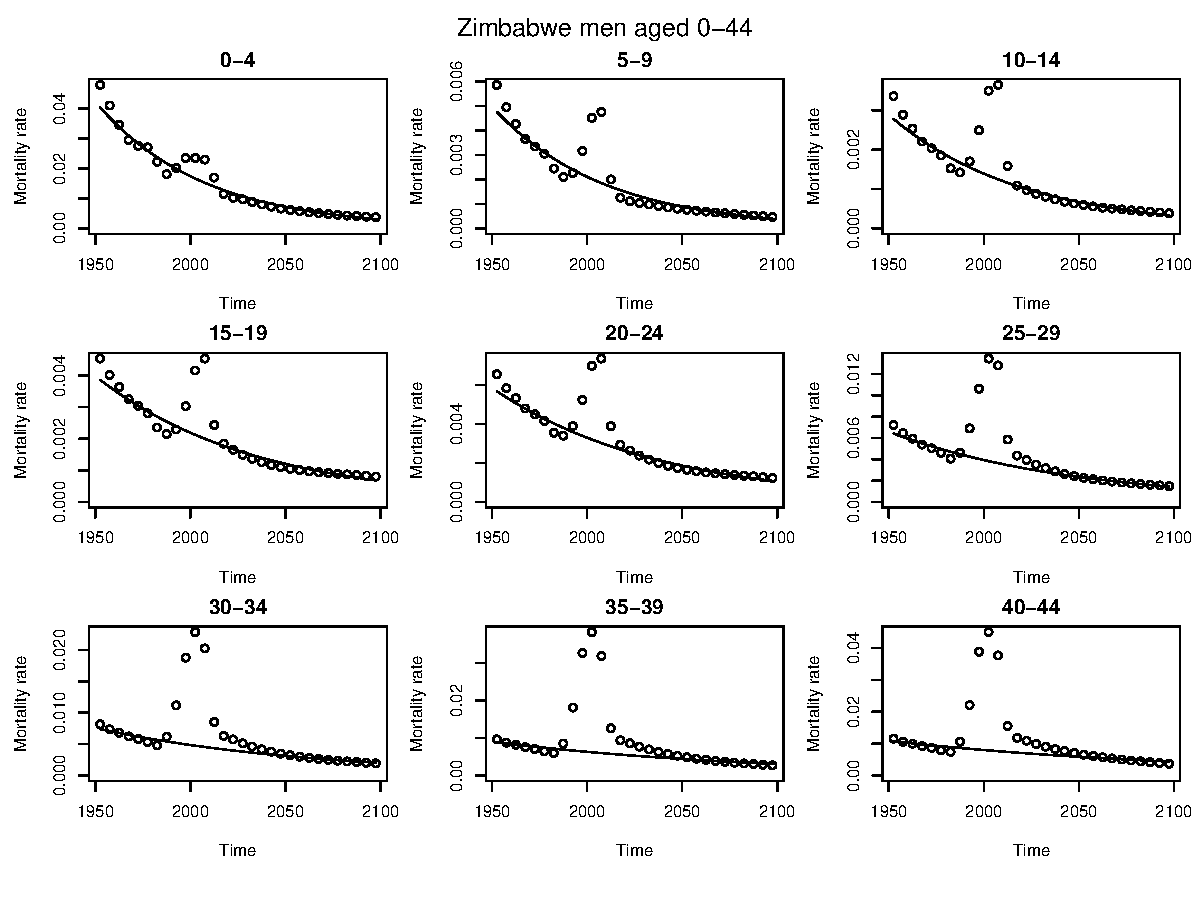
\includegraphics[width=16cm,height=16cm]{EstimatingRatesFromUNPDv2-MortalityMen1} 

\caption{Mortality rates for men over time by 5 year age groups. Circles show UNPD estimates (including HIV mortality), lines show estimate based on a log-linear model for each age group.}
\label{Mortalitymen1}
\end{figure}


\begin{figure}
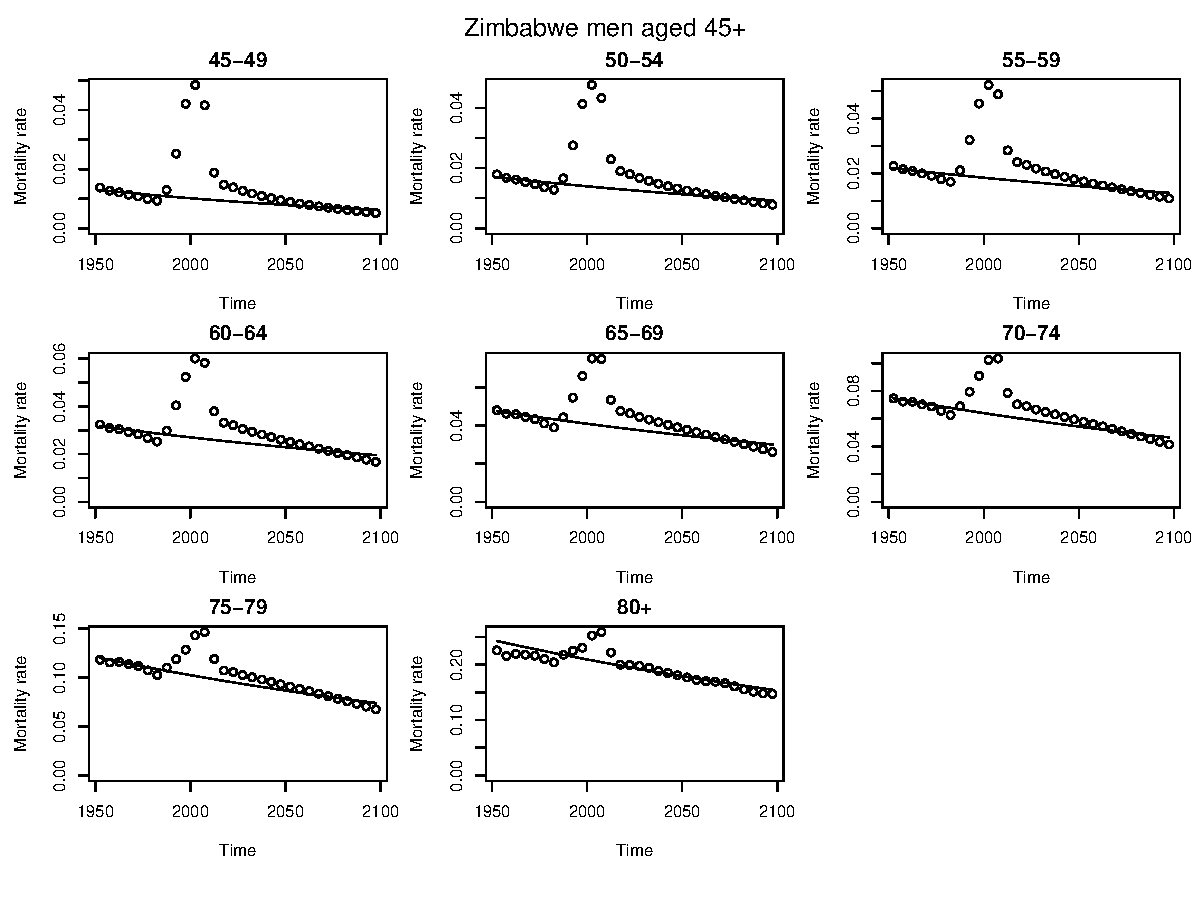
\includegraphics[width=16cm,height=16cm]{EstimatingRatesFromUNPDv2-MortalityMen2} 

\caption{Mortality rates for men over time by 5 year age groups (cont). Circles show UNPD estimates (including HIV mortality), lines show estimate based on a log-linear model for each age group.}
\label{Mortalitymen1}
\end{figure}


\begin{figure}
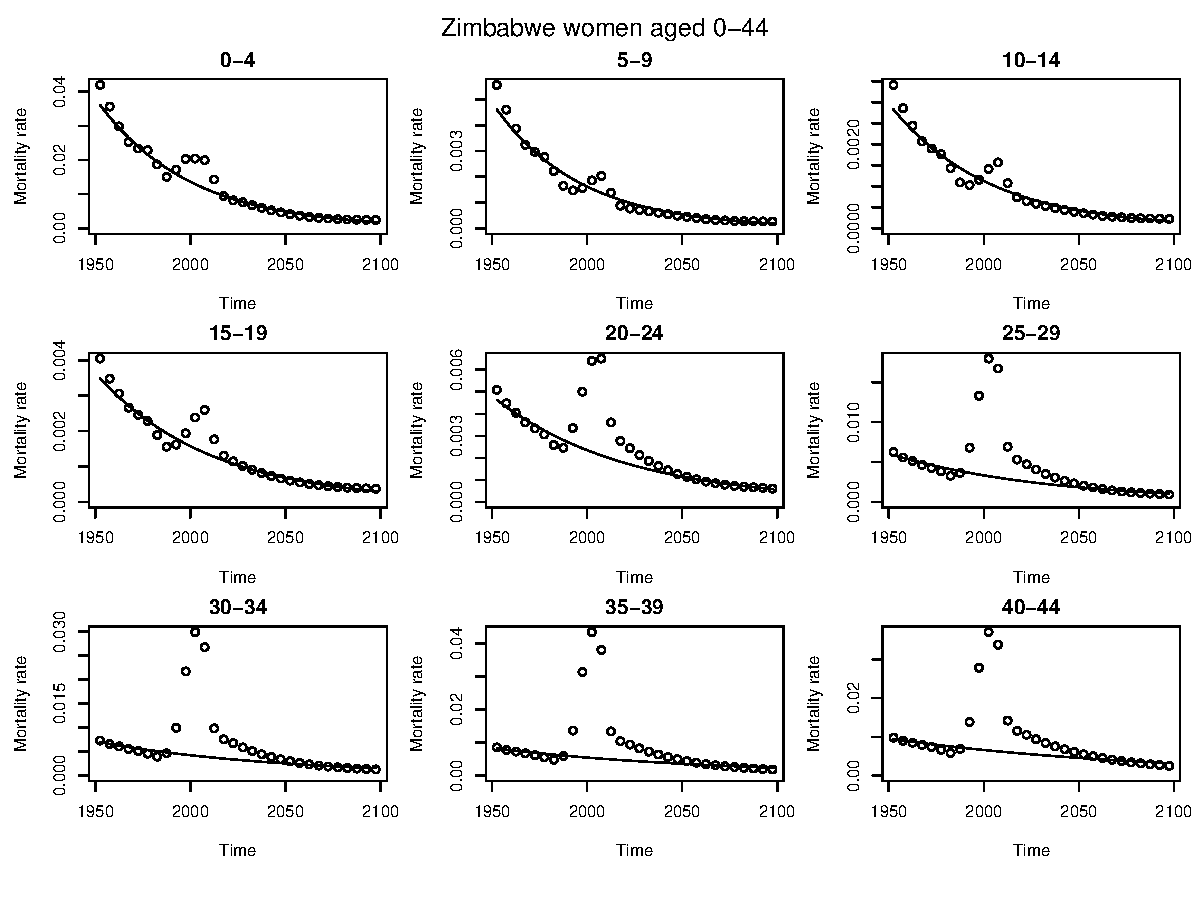
\includegraphics[width=16cm,height=16cm]{EstimatingRatesFromUNPDv2-MortalityWomen1} 

\caption{Mortality rates for women over time by 5 year age groups. Circles show UNPD estimates (including HIV mortality), lines show estimate based on a log-linear model for each age group.}
\label{Mortalitywomen1}
\end{figure}


\begin{figure}
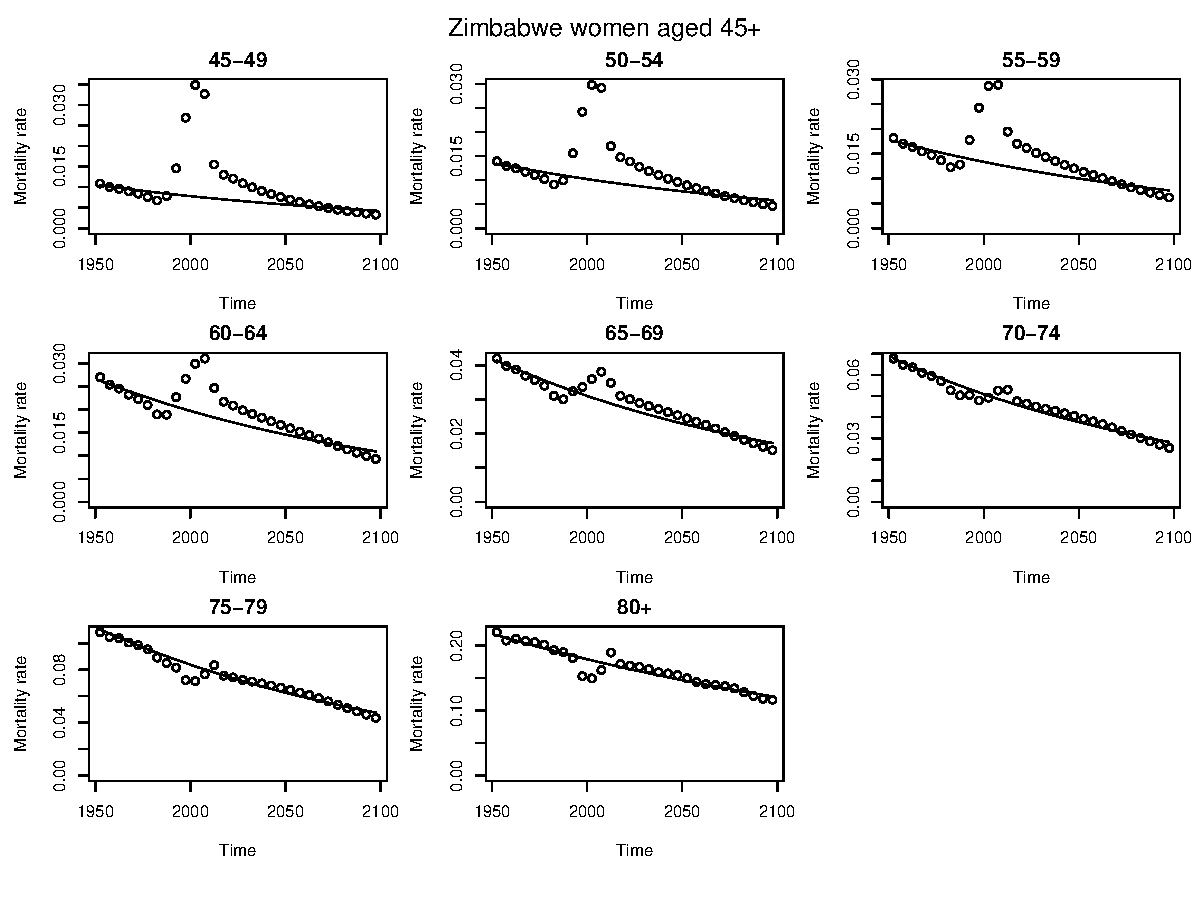
\includegraphics[width=16cm,height=16cm]{EstimatingRatesFromUNPDv2-MortalityWomen2} 

\caption{Mortality rates for women over time by 5 year age groups (cont). Circles show UNPD estimates (including HIV mortality), lines show estimate based on a log-linear model for each age group.}
\label{Mortalitywomen1}
\end{figure}



\clearpage

\begin{landscape}
% latex table generated in R 3.6.0 by xtable 1.8-4 package
% Tue Jul  2 04:52:15 2019
\begin{table}[ht]
\centering
\begin{tabular}{rrrrrrrrrrrrrrrrrr}
  \hline
 & 0-4 & 5-9 & 10-14 & 15-19 & 20-24 & 25-29 & 30-34 & 35-39 & 40-44 & 45-49 & 50-54 & 55-59 & 60-64 & 65-69 & 70-74 & 75-79 & 80+ \\ 
  \hline
Intercept & 33.81 & 36.65 & 30.42 & 21.22 & 20.46 & 20.59 & 19.29 & 18.13 & 17.45 & 15.40 & 13.45 & 12.66 & 11.51 & 10.72 & 10.33 & 9.75 & 6.15 \\ 
  Coeff & -0.02 & -0.02 & -0.02 & -0.01 & -0.01 & -0.01 & -0.01 & -0.01 & -0.01 & -0.01 & -0.01 & -0.01 & -0.01 & -0.01 & -0.01 & -0.01 & -0.00 \\ 
   \hline
\end{tabular}
\caption{Parameters for Zimbabwe men mortality} 
\end{table}% latex table generated in R 3.6.0 by xtable 1.8-4 package
% Tue Jul  2 04:52:15 2019
\begin{table}[ht]
\centering
\begin{tabular}{rrrrrrrrrrrrrrrrrr}
  \hline
 & 0-4 & 5-9 & 10-14 & 15-19 & 20-24 & 25-29 & 30-34 & 35-39 & 40-44 & 45-49 & 50-54 & 55-59 & 60-64 & 65-69 & 70-74 & 75-79 & 80+ \\ 
  \hline
Intercept & 35.62 & 40.31 & 34.72 & 28.14 & 25.03 & 23.65 & 23.13 & 21.46 & 19.04 & 16.63 & 15.41 & 15.72 & 15.72 & 15.10 & 14.28 & 13.28 & 8.15 \\ 
  Coeff & -0.02 & -0.02 & -0.02 & -0.02 & -0.02 & -0.01 & -0.01 & -0.01 & -0.01 & -0.01 & -0.01 & -0.01 & -0.01 & -0.01 & -0.01 & -0.01 & -0.01 \\ 
   \hline
\end{tabular}
\caption{Parameters for Zimbabwe women mortality} 
\end{table}

\end{landscape}


%%%%%%%%%%%%%%%%%%%%%%%%%%%%%%%%%%%%%%%%%%%%%%%%
%
%%%%%%%%%%%%%%%%%%%%%%%%%%%%%%%%%%%%%%%%%%%%%%%%
\begin{Schunk}
\begin{Sinput}
> # Writing out mortality rates:
> write.table(rbind(mortality.coeffs.men,mortality.coeffs.women),file=paste0(country.no.spaces,"_mortalityByAgeCoefficients.txt"),row.names=FALSE,col.names=FALSE)
> 
\end{Sinput}
\end{Schunk}

\clearpage

\section*{Fertility rates}





\begin{figure}
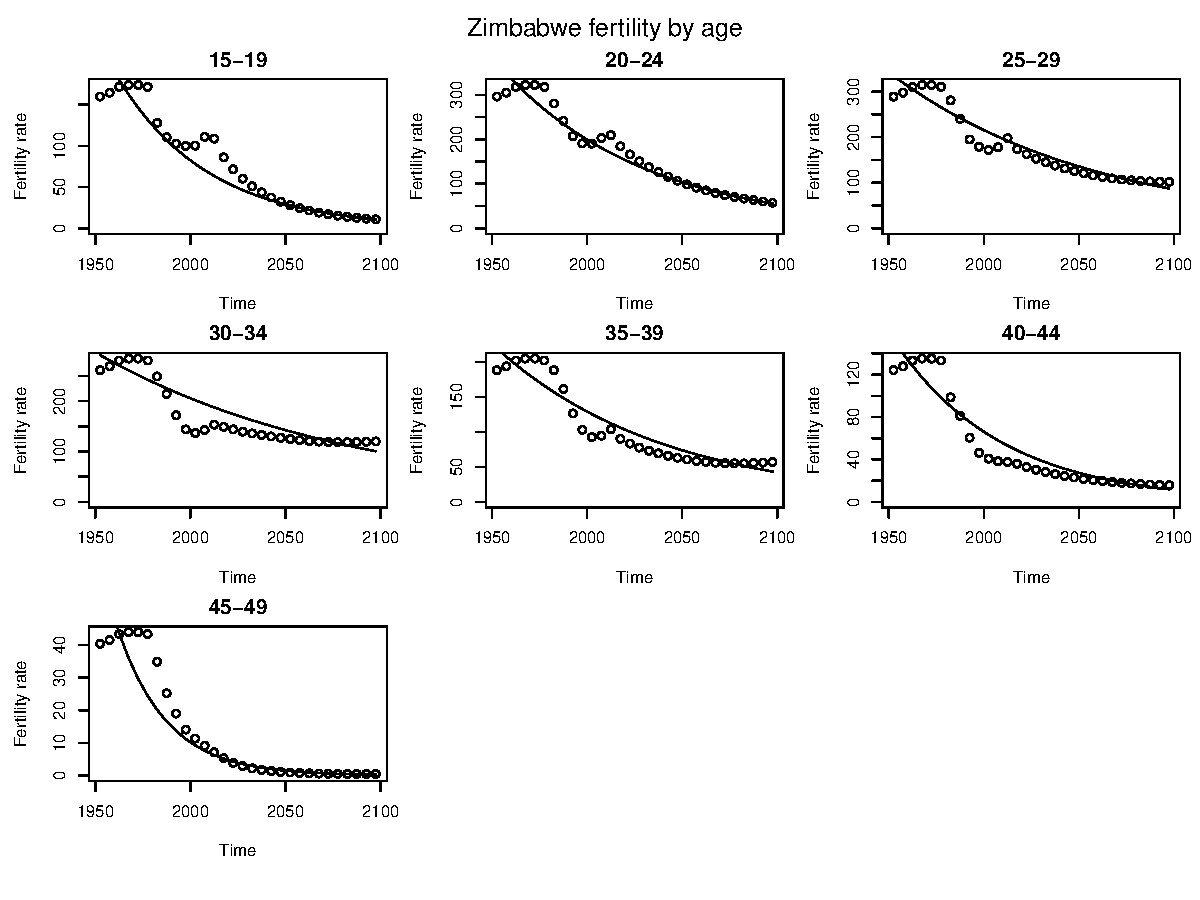
\includegraphics[width=16cm,height=16cm]{EstimatingRatesFromUNPDv2-Fertility} 

\caption{Fertility rates for women  over time by 5 year age groups. Circles show UNPD estimates (which are adjusted for the effects of HIV), lines show estimate based on a log-linear model for each age group.}
\label{Fertility}
\end{figure}


\clearpage
\section*{Experiments}
%%%%%%%%%%%%%%%%%%%%%%%%%%%%%%%%%%%%%%%%%%%%%%%%
% EXPERIMENT: Trying to see if a 2d function fits OK: 
%%%%%%%%%%%%%%%%%%%%%%%%%%%%%%%%%%%%%%%%%%%%%%%%

\begin{figure}
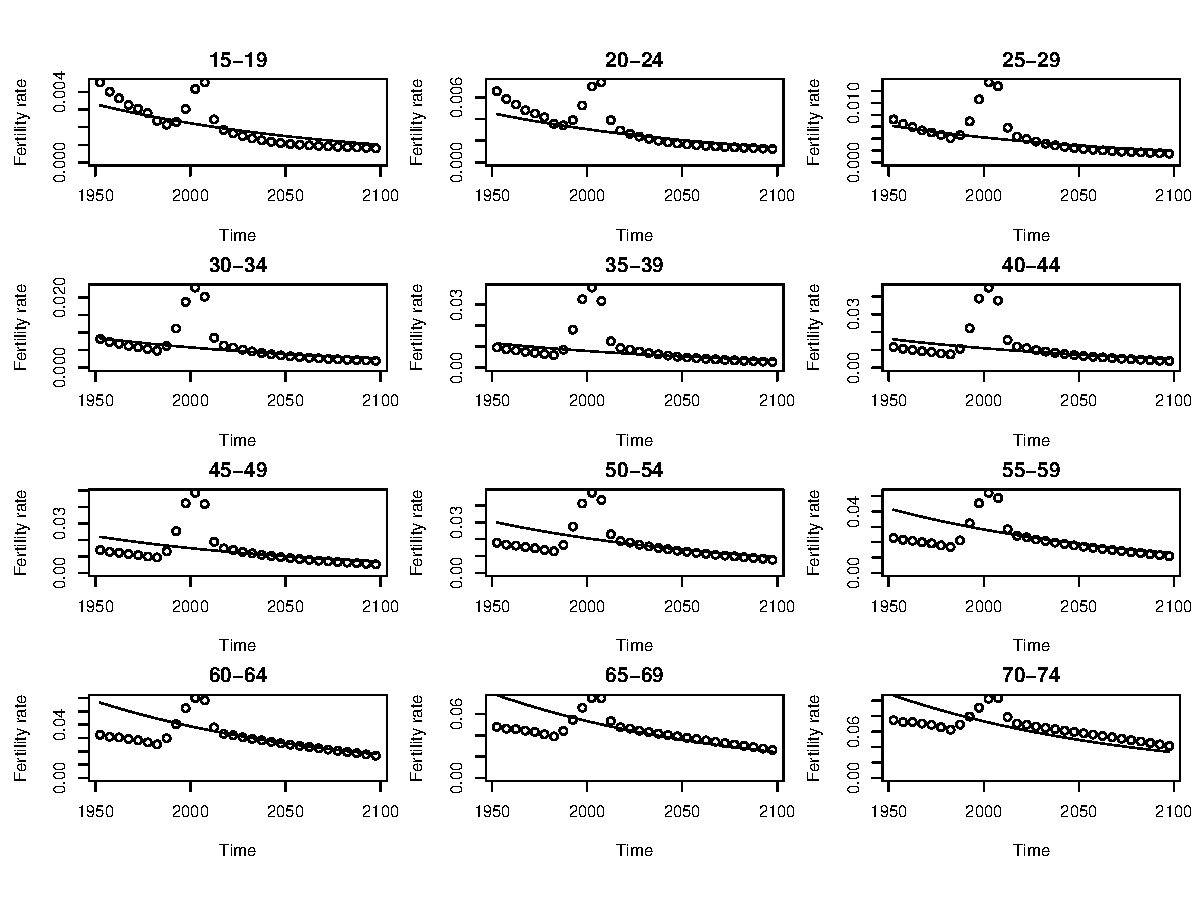
\includegraphics[width=16cm,height=16cm]{EstimatingRatesFromUNPDv2-Testmortality2d} 

\caption{Experiment for men to see if we can fit a 2d function - ie a single regression by age group and time for each gender and country -  well for mortality. For now I think we should stick with the different regressions for each age group.}
\label{ExperimentSingleRegression}
\end{figure}

\section*{Discussion}

For mortality rates we need to have some way of discounting HIV mortality. I think that fitting a function separately to each age group  - and ignoring the periods when HIV mortality is high - gives an OK fit. It seems to me that we can't fit a 2d model by age and time (assuming independence between the 2) as well. As mortality is something in the background, validated against age distribution at different time points, I think we can ignore the parametric complexity and just input them as fixed quantities.

For fertility it is not clear that any function will fit this well. For now we can use the UNPD numbers directly.

\end{document}
